\clearpage
\onecolumn
\appendices
\section{Design Appendix}

% Figure~\ref{fig:settings} shows the settings page of \toolname.

\begin{figure*}[!h]
    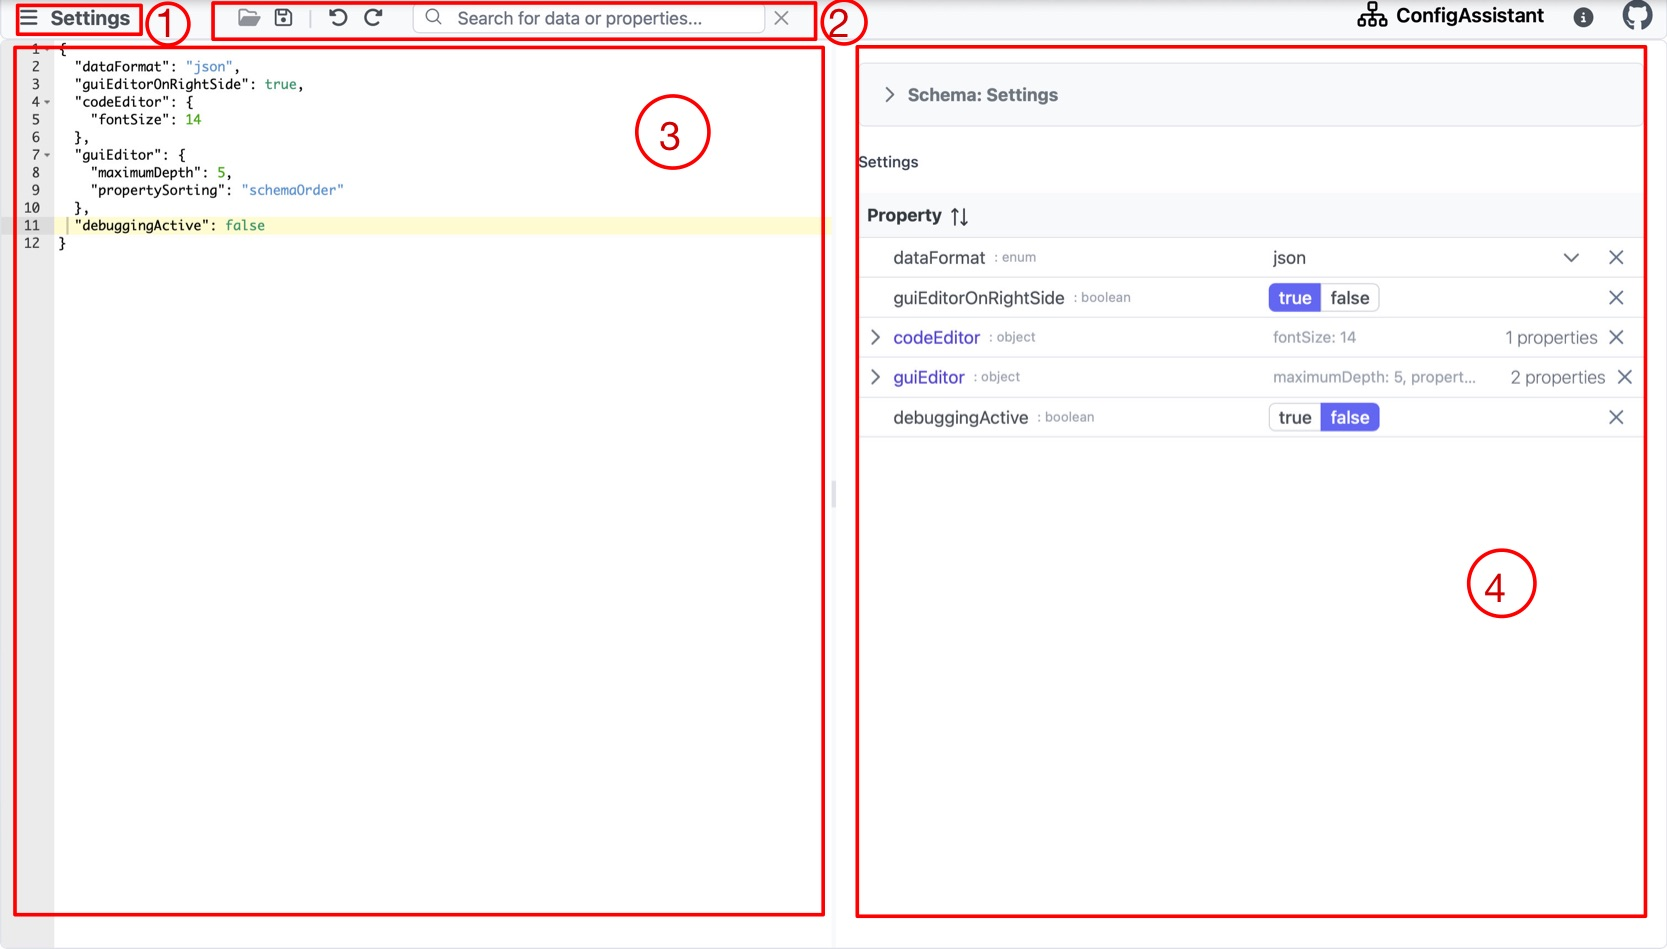
\includegraphics[width=\textwidth]{figures/settings}
    \caption{UI of the Settings view}
    \label{fig:settings}
\end{figure*}



% Minye


\section{User Study Appendix}

\begin{table*}[!htbp] %keyuri
    \centering
    \caption{User Study 1 - Feedback and Solution}
    \label{table:user_study1}
    \begin{tabular}{p{0.45\linewidth}p{0.45\linewidth}}
        \toprule
         \thead{Feedback} & \thead{Solution} \\
        \midrule
        The property value should not be autocorrected if the user enters an incorrect value.
        Instead, an error message or another way should be used to inform the user that their input is incorrect.
        &
        Instead of autocorrecting values, we now provide more clear user feedback on incorrect values (red underline, error symbol). \\
        \midrule
        It would be good to have the ability to remove data entries with the GUI panel.
        &
        Implemented by adding a \textit{remove} button next to properties that have data and are not required. \\
        \midrule
        A search functionality to locate properties would be helpful, especially within nested levels.
        & Implemented in the toolbar.
        All findings are highlighted in the GUI panel. \\
        \midrule
        %& 4. The Schema editor GUI panel contains extensive metadata, but the code editor panel remains empty. & 4. bla bla bla \\
        %\midrule
        The GUI panel feels overwhelming to the user due to many variations in the styling and color of the GUI elements.
        &
        We slightly reduced the number of different styles by no longer showing required properties in boldface and instead just showing an asterisk next to it. \\
        \midrule
        The cursor should not have the clickable animation when hovering over non-clickable fields in the GUI editor.
        &
        Now we only show the clickable animation when hovering over clickable GUI components. \\
        \midrule
        In drop-down menus, we do not need a button to clear the selection.
        &
        We disabled the option of clearing the selection. \\
        \midrule
        If the type of a property is ``any'', it should not be interpreted as the ``string'' type in the GUI panel.
        &
        We improved the representation of the ``any'' type, but further improvements are needed, which will be considered in future work.\\
        \midrule
        Validation errors should not be highlighted via a warning symbol, but instead an error symbol.
        &
        We changed the warning symbol into an error symbol. \\
        \midrule
        After performing an undo or redo action, the cursor should jump to the corresponding location to reflect the changes made by the user.
        &
        This will be considered in future work. \\
        \bottomrule
    \end{tabular}
\end{table*}


\begin{table*} %keyuri

    \centering
    \caption{User Study 2 - Feedback and Solution}
    \label{table:user_study2}
    \begin{tabular}{p{0.45\linewidth}p{0.45\linewidth}}
        \toprule
        \thead{Feedback} & \thead{Solution} \\
        \midrule
        A graph-based view would be more intuitive for handling complex data structures.
        &
        This will be considered in future work. \\
        \midrule
        Providing immediate feedback to users when they enter incorrect ranges is essential to prevent them from inputting invalid values into the property.
        &
        We now highlight schema violations by a red error symbol in the GUI panel and underlining the property name in red.
        Additionally, the tooltip lists all schema violations of a property. \\
        \midrule
        Validation errors should also be reflected in the GUI panel, including for child properties.
        &
        See the point above.
        Also, now the tooltip lists schema violations of child properties. \\
        \midrule
        When dealing with an array, the display name of array elements (index) should be improved.
        Currently, the tool only shows the element index.
        &
        We replaced the numerical labels with a standard programming notation, which is \texttt{propertyName[0]}, \texttt{propertyName[1]}, \ldots
        \\
        \midrule
        The input field next to the \textit{Add Item} button is confusing.
        Both the input field and the button can be used to create a new item, which is redundant.
        &
        We removed the input field next to the button. \\
        \midrule
        It would be more consistent if all user input in the GUI panel was within the right column of the table.
        In some scenarios user input is needed within the left column (for names of new properties), which feels inconsistent.
        &
        Because of the nature of JSON schema, we retained the property name within the left column.
        To make it clear to the user that the property name can be edited, we added an \textit{edit} icon next to it. \\
        \midrule
        The search function for locating specific properties lacks clarity at first glance.
        It should provide an immediate response and extend to nested levels, rather than merely highlighting the higher-level findings.
        &
        The search now provides a list of results, and upon clicking on a particular result, it jumps to that result in the code panel and GUI panel.
        In the GUI panel, if the element is nested, its parents will be automatically expanded. \\
        \bottomrule
    \end{tabular}

\end{table*}

\begin{table*} %keyuri
    \centering
    \caption{User Study 3 - Feedback and Solution} \label{table:user_study3}
    \begin{tabular}{p{0.45\linewidth}p{0.45\linewidth}}
        \toprule
        \thead{Feedback} & \thead{Solution} \\
        \midrule
        Working with the schema editor is difficult for me.
        It does not feel intuitive.
        &
        We made the schema editor more intuitive by creating our own simplified JSON schema meta schema.
        For example, advanced JSON schema features are separated from the simple ones.
        See section~\ref{subsec:schema-editor} \\
        \bottomrule

    \end{tabular}

\end{table*}

\begin{table*} %keyuri
    \centering
    \caption{User Study 4 - Feedback and Solution} \label{table:user_study4}
    \begin{tabular}{p{0.45\linewidth}p{0.45\linewidth}}
        \toprule
        \thead{Feedback} & \thead{Solution} \\
        \midrule
        Modifying or renaming a new property in the GUI panel does not appear to take effect when double-clicking on it.
        &
        Renaming properties in the GUI panel can now be done using the \textit{edit} button next to the property name. \\
        \midrule
        When creating a new property in the schema editor, its sub-schema has to be selected, such as \textit{string property} or \textit{boolean property}.
        Additionally, the type of the property has to be selected by the user too.
        Therefore, for example, when creating a new \textit{string property}, the user has to select that it is a string two times.
        It would be much more intuitive if the selection needs to be done only one time.
        & We completely overhauled our JSON schema meta schema.
        Now, when creating a new property, the user will have to select the type only once. \\
        \midrule
        A toggle button should be implemented to enable and disable the code panel and GUI panel.
        & Only having a GUI panel or only having a code panel restricts the user unnecessarily.
        The interplay of both panels is what makes this tool most effective.
         If the user does not want to use one of the panels, they can resize that panel to a very small size.  \\
        \midrule
        When working with a particular property in the GUI panel, the opacity of the other properties should be decreased, visually highlighting the currently focused property.
        & Will be considered in future work. \\
        \midrule
        Simplify the schema editor to make it easier to work with, for those who are not very familiar with JSON schema.
        &
        Has been done, see section~\ref{subsec:schema-editor}. \\
        \bottomrule

    \end{tabular}

\end{table*}

\begin{table*} %keyuri

    \centering
    \caption{User Study 5 - Feedback and Solution} \label{table:user_study5}
    \begin{tabular}{p{0.45\linewidth}p{0.45\linewidth}}
        \toprule
        \thead{Feedback} & \thead{Solution} \\
        \midrule
        The search button is not immediately evident, making it challenging for users to locate the search function. &
        Instead of showing the search bar only when clicking the search button, we now always show it. \\
        \bottomrule

    \end{tabular}

\end{table*}
